\chapter{AN EVOLUTIONARY ALGORITHM FOR GENERATING PARETO EFFICIENT POTENTIALS}
\label{ch:methodology}

The purpose of this chapter to introduce a cost-efficient algorithm to determine the appropriate trade-offs between concurrent minimization problems associated with several critera.

Our algorthm has the following goals: (1) to identify the strengths and weaknesses of solution of the Pareto optimal solutions, (2) to generate estimates of the Pareto optimal front in a serious of iteratively better approximations, and (3) to describe the candidate parameterizations through the use of a distribution function and use Monte Carlo sampling, but updating the distribution by keeping the Pareto dominated points.

In the development of this evolutionary algorithm, some of the techniques used in genetic algorithims and evolutionary algorithms are consciously not implemented.  In GA techniques, the population samples are fixed and evolve based upon criteria, which in our case might be spurious.  The end state of this algorithm is identify probability distributions which produce Pareto optimal results, which could be used follow up efforts to integrate this algorithm into existing and well-defined UQ methodologies.

\begin{figure}[ht]
	\centering
  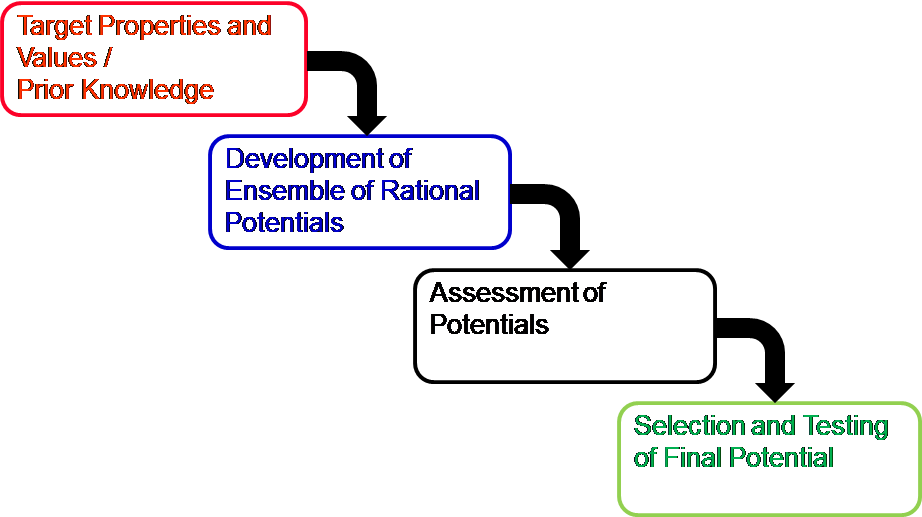
\includegraphics[width=0.8\textwidth]{chapter5/fig_pareto_schematic}
  \caption{Schematic of the approach taken to potential development.}
  \label{fig:pareto_schematic}
\end{figure}


Figure \ref{fig:pareto_schematic} shows a schematic of the approach to the development of potentials outlined here. There are essentially four steps.
(i) The identification of structures, properties and their values to be used in the potential fitting. The specific values can be taken from experiment, from higher fidelity calculation methods such as quantum chemical or density functional theory (DFT) calculations, or a combination thereof. Our approach in this step is similar to standard potential development approaches.
 (ii) The use of ideas from Pareto optimization to develop an ensemble of rational potentials. The term ‘rational’ will be discussed in detail below, but involves the use of a simple algorithm to identify potential parameterizations that make sense to consider further. This is the central idea of our approach and is very different from a conventional potential fitting approach
(iii) The analysis of the ensemble of rational potentials to identify features and clustering in both the high-dimensional parameter space and in the high-dimensional space of errors in the predictions of the properties.
(iv) The down-selection and testing of a few parameterizations or a single parameterization of the potential for use in further simulations.
We focus mainly on the second of these steps: the development of an ensemble of rational potentials. We do, however, briefly discuss the other three parts of the process.


\section{Incorporation of Prior Information}

In taking a new approach to potential optimization, we recall the fundamental challenge, which is the multi-objective optimization problem of minimizing the errors in a large number, $N_Q$, of QOIs, in this case the absolute difference between the predicted material properties, $\bm{q}$, and the target values, $q_i$.  If  $\hat{V}(\bm{\theta})$ is an interatomic potential parameterized by the vector $\bm{\theta} = (\theta_1,...,\theta_{N_P})$ with $N_P$ parameters, then predicted material properties becomes $\hat{\bm{q}}(\bm{\theta}) = (\hat{q}_1,...\hat{q}_{N_Q})$.  Using the absolute loss function for our choice of objective functions, then the problem becomes the minimization of  $\bm{L}(\bm{\theta}) = (|\hat{q}_1-q_1|,...|\hat{q}_{N_Q}-q_{N_Q}|)$, simulatenously.  The optimization problem we thus face is minimizing each objective function in $N_Q$ target properties described by a fixed functional form with $N_P$ parameters.  That is, both error space and parameter space typically have high dimension.


\subsection{Prior distribution}

For existing formalisms, one can incorporate parameter information from existing potentials.  For each parameter, define an uppper and lower bound to define the uniform distribution.  Having a uniform prior means that the probability density is constant over its support defined as $\theta_{i}^{\text{min}} \leq \theta_i \leq \theta_{i}^{\text{max}}.$  A uniform prior doesn't favor any particular value of $\theta_i$, since it supposes that all values in the range are equally likely.

In the case, where the initial parametric uncertainty cannot be bound.  The Jefferies prior is another approach for representing ignorance in priors for continuous variables.
Strictly speaking, the use of uniform priors are optimal and we logically can show that our prior information for $\bm{theta}$ must be identical over it's support.  However, complete ignorance about the probability for a parameter may not be true.

Based upon application, different probability distribution functions to represent prior knowledge.  For example, a known potential

\subsection{Parametric Constraints}

As demonstrated in \ref{ch:potential_development}, scalarization techniques to implement inequality and equality constraints requires defining the Lagrangian for the constrained optimization problem, which complicates the implementation process.

simply defining upper and lower bounds for each parameter, and sampling from a uniform distribution between these bounds; such a distribution is known as an uninformed, or vague, distribution.  In doing this, we may be able to apply some constraints, such as the values of certain parameters are strictly positive.

\subsection{Qoi Constraints}

\section{Probabilistic Optimization}

\subsection{Inadeuqacy of a Bayesian Appproach}
In a Bayesian approach, the Bayes estimator is an estimator that minimizes the posterior expected value of a loss function, (i.e. the posterior expected losss).

\subsection{Sampling distribution}
The process described here combines Popper's propensity interpretation of probability with Bayesian concepts in which to refine our distribution function.  The process described here uses many concepts and notation from Bayesian inference, covered in section \ref{section:bayes}, but is adapted for our process here.  Popper noted that the outcome of a physical experiment is produced by a certain set of "generating conditions". When an experiment is repeated, we really perform another experiment with a similar set of generating conditions. To say that a set of generating conditions has propensity $p$ of producing the outcome $E$ means that those exact conditions, if repeated indefinitely, would produce an outcome sequence in which $E$ occurred with limiting relative frequency $p$. For Popper then, a deterministic experiment would have propensity $0$ or $1$ for each outcome, since those generating conditions would have the same outcome on each trial. In other words, non-trivial propensities (those that differ from $0$ and $1$) only exist for genuinely indeterministic experiments.

Here the prior distribution function are the propensities associated that a particular parameterization is Pareto optimal.  In the deterministic approach outlined \ref{ch:potential_development}, $\bm{\Theta}^*$ is the Pareto set.  Here $\bm{\Theta}$ is a random variable, with $\bm{\theta} \in \bm{\Theta}$ being a single realization of that random variable defined by the prior probability distribution function, which is our current best estimate that the probability distribution function produces parameterizations in the Pareto set.  The prior density function is the generator of parameterizations, which can then be used into computational experiments which are then amenable to frequentist approaches to density estimation.

The sampling distribution, which is defined as the likelihood in Bayesian literature, is the distribution of the material properties conditional on the parameters, i.e. $p(\hat{\bm{q}}|\bm{\theta})$.  Instead of analytically determining $p(\bm{\hat{q}}|\bm{\theta})$, we sample from the prior distribution of $\bm{\theta}$.  To determine the sampling distribution, treat $\bm{\theta}$ as the random variable $\bm{\Theta}$.   Since $\bm{q}(\bm{\theta})$ is non-analytic, a representative sample is constructed from which the probability distribution can be estimated.  In the context of Popper, the prior distribution is not useful other than in which to conduct computational experiments.

The process of sampling by generating variates of a probability distribution function was covered in Chapter \ref{ch:probability},
In a sampling process, constraints on the parameter space are incorporated into the sampling procedure, by rejecting

Accounting for equality constraints requires modification of the sampling procedure.  A typical technique used in simulation methdology comes from drawing random variates from a standard multi-variate normal distribution, as discussed in \ref{section:multivariate_sampling}  By definition, an equality constraint imposes a correlation coefficient of unity to an off-diagonal term, which breaks Cholesky decomposition of the covariance matrix.

Our treatment of the mapping of the empirical potential is treated as a bijective mapping into two measure spaces.
In scalar optimization problems, random sampling are ubiquituous for global minimization, including techniques such as simulated annealing[20], genetic algorithms[21], tabu search [22]–[24], and multi start[25].  Although these approaches require a large number of samples, they do not require a priori knowledge of the objective function to achieve the global mimima..  Here we take the approach of generating a large number of parameter sets through random sampling of the parameter space, and algorithmically determining if these candidate potentials are optimal in a multi-objective optimization sense.  The algorithmic approach we take is centered on the idea of Pareto optimality.

Let us define parameter space with the probability measure space $(\Theta,\mathcal{F}(\Theta),\mathbb{P})$.

Then we define the error space of the structure property relationships with the probability measure space $(\mathcal{E},\mathcal{F}(\mathcal{E})),\mathbb{Q})$.

To solve forward problems, the parameters of a potential, $\bm{\theta}$ is known \emph{a priori}, are used in conjunction of a set of atomic arrangements in a simulation cell with periodic boundary conditions to predict $n$ material properties, $\bm{q} = (q_1,...q_n)$.  These predictions depend not only on the atomic arrangements but also on the parameterization, denoted
$\bm{\hat{q}}(\bm{\theta}) =
    (\hat{q}_1(\bm{\theta}),...\hat{q}_n(\bm{\theta}))$.
The differences between the predicted values and references values are denoted
$\bm{\epsilon}(\bm{\theta}) =
    \lvert \bm{\hat{q}}(\bm{\theta})
         - \bm{q}_i
    \rvert$,
where $|\bm{x}|$ is the elementwise magnitude of the vector $\bm{x}$.

The problem of parameterization is an inverse problem where an optimal parameterization produces ideal outcomes for the forward problem, i.e. difference between the predicted value and the reference value,
$\epsilon_i(\bm{\theta}) = 0$.
Since replication of results is typically not achievable, then the goal of parameterization becomes
$\min_{\bm{\theta}} \epsilon_i(\bm{\theta})$
for all $i$.  Typically, there does not exist an optimal parameterization, $\bm{\theta}^*$, which minimizes $\epsilon_i(\bm{\theta})$ for all $i < n$.  Requiring a prioritization of which material properties have a preference for fidelity in predictions.

The typical approach to solving the inverse problem transforms the above problem into a scalar optimization problem amenable to derivative approaches.  A cost function $C$ which couples the individual objectives, $\epsilon_i$, along with a set of weights $\bm{w} = (w_1,...,w_n)$, to represent preferences, that is
\begin{equation}
    C(\bm{\theta}) = \sum_i^n w_i (\hat{q}_i(\bm{\theta}) - q_i)^2
                   = \sum_i^n w_i \epsilon_i^2(\bm{\theta})
\end{equation}

It is clear that the selection of $\bm{w}$ uniquely determines $\bm{\theta}^*$.  However, the values of $w_i$ which will produce an acceptable potential are typically not known \emph{a priori}.  When the initial weighting scheme fails to give an acceptable results, $\bm{w}$ is changed in an \emph{ad hoc} approach until an acceptable parameterization is achieved.

Since analytical solutions are intractable, numerical solutions are achieved by selecting an initial parameterization, $\bm{\theta}_0$, and using derivative-based optimization techniques to minimize the cost function.  If the $C(\bm{\theta})$

\subsection{Partitioning}

As the number of free parameters increase, the size of the sampling space increases exponentially.

Partitioning is the task of decomposing the parameterization problem into subproblems.  Decomposition is performed to reduce the problem size.  This concept is common in the the development of multi-component potentials.   For example, in alloy potentials a potential parameterization can be used in  As identified by Martinez \emph{et al.},

\begin{equation}
    \Theta = \Theta_0 \supset \Theta_1 \supset \hdots \supset \Theta_k = \Theta^{(p)}
\end{equation}

which produces due to Eq %\ref{eqn:def_Q} and \ref{eqn:def_E}

\begin{equation}
    \mathcal{E} = \mathcal{E}_0 \subset \mathcal{E}_1 \supset \hdots \supset \mathcal{E}_k = \mathcal{E}^{(p)}
\end{equation}

for $k < \infty$ iterations.  Since $\Theta \subset \mathbb{R}^p$ and $\mathcal{E} \subset \mathbb{R}^n$, we provide the following approach which uses Monte Carlo simulation in an approach which is inspired by Bayesian inference, although this approach does not use a Bayesian updating approach.  The goal of this approach is to produce an ensemble of $\bm{\theta}\in \Theta^{(p)}$ and describe this ensemble as a probability distribution which could be used as a starting point in uncertainty quantification propagation.

\section{The Problem}

Using the construction of an empirical potential as outlined in Chapter 2, we define an empirical interatomic potential, $\hat{V}$, which approximates the potential energy surface, $V$.
If $\bm{R}$ is an atomic configuration, then both the EIP and the PES maps the configurational space onto energies, $\hat{V}:\bm{R} \rightarrow \mathbb{R}$ and $V:\bm{R} \rightarrow \mathbb{R}$.
We can then write
\begin{equation}
    \hat{V})(\bm{R}) = V(\bm{R}) + \epsilon(\bm{R})
\end{equation}
where $\epsilon(\bm{R})$ is a difference equation required for equality balance.
\begin{equation}
    \epsilon(\bm{R}) = \hat{V}(\bm{R}) = V(\bm{R})
\end{equation}
Since ${\epsilon \rightarrow 0}$ as the EIP becomes a better approximation to the PES, we will use $\epsilon$ to define loss functions and performance filters.

If $\hat{V}$ is an analytical parameterized by $P$ parameters, $\bm{\theta}=[\theta_1,...,\theta_P]\in\mathbb{R}^P$

\section{A Probability Approach}

In a deterministic approach, a parameterization, $\theta$, is a member of the domain $\Theta$, and we use numerical routines to identify the optimal parameterization $\theta^*\in\Theta$.

Here we take a probabilistic approach to potential development.
Here $\Theta$ is a random variable, and $\theta\in\Theta$ is a specific realization of that random variable.

For the purpose of generality, we use $\hat{V}$ to predict a set of material values $\hat{q}$ from which we have target values $\bm{q}\in\mathbb{R}$


We replace the notion of $\theta$ being a deterministic value, and instead $\theta\in\Theta$

\section{The Fitting Database}

\section{An Iterative Procedure}
We propose the following approach:
%\begin{subequations}
\begin{equation}
	\Theta_k \rightarrow \hat{Q}_k(\Theta_k) \rightarrow \mathcal{E}_k(\Theta_k)
\end{equation}
\begin{equation}
	\mathcal{E}_k(\Theta_k) \rightarrow \mathcal{E}_k^{(p)}(\Theta_k^{(p)})
\end{equation}
\begin{equation}
	\mathcal{E}_k^{(p)}(\Theta_k^{(p)}) \rightarrow \mathcal{E}_k^{(cp)}(\Theta_k^{(cp)})
\end{equation}
\begin{equation}
	      \mathcal{E}_k^{(cp)}(\Theta_k^{(cp)}) \rightarrow \Theta_{k+1}
\end{equation}
%\end{subequations}
% this paragraph has some notational abuse, but is used for the sake of clarity rather than making the notation mathematical rigorous.
The notation $\rho(\bm{\theta})$ refers to the joint probability density function that $\bm{\theta} \in \Theta^{P}$.
Intuitively, one can think of
$\rho(\bm{\theta})\Delta\bm{\theta}$
as the probability that a random variable drawn from $\rho(\bm{\theta})$ will fall within the infinitesimal compact set $[\bm{\theta},\bm{\theta}+\Delta\bm{\theta}]$

Even if $\Theta$ is defined as compact, $\hat{Q}$ may not be bounded.  By construction $\hat{q}_i > 0 $, however $\hat{q}_i$ may not be bounded from above.  There exists $\bm{\theta} \in \Theta$ which produces pathological members of the Pareto set.  Specifically, there is exists $\bm{\theta} \in \Theta$ such that $\bm{\epsilon}(\theta) \in \mathcal{E}^(p)$, but produces an $\epsilon_i(\bm{\theta}) > \epsilon_{i,max}$ for at least one $i\in\{1,...,n\}$, where $\epsilon_{i,max}$ is an arbitrary performance requirement.

We generalize Eq
To estimate $\Theta^{(p)}$, we simplify the drawing of samples from a uniform distribution defined by hyperrectangles which defines $\Theta$The choice of
\subsubsection{Kernel Density Estimate}

The Kullbach-Leiber divergence\cite{kullback1951_kld} measures the divergence between two probability density functions $f(x)$ and $g(x)$,
\begin{equation}\label{eq:kld}
   D(f \parallel g) = \int f(x) \log \frac{f(x)}
                                          {g(x)} dx
\end{equation}
is commonly used in statistics as a measure of similarity between two density distributions, and has the following properties: (1) self-similarity, $D(f \parallel f) = 0$, (2) self-identification, $D(f \parallel g) = 0$ only if $f=g$, and (3) positivity, $D(f \parallel g) \geq 0$ for all $f$ and $g$.

The integral in Equation \ref{eq:kld} can be calculated from Monte Carlo\cite{hershey2007_kld_approx}, by drawing a sample $x_i$, from the statstical distribution of $f$ such that $\mathbb{E}\left[\log\frac{f(x)}{g(x)}\right] = D(f \parallel g)$.  Using $N$ i.i.d. samples $\left\{x_i\right\}_{i=1}^N$, we have
\begin{equation}
  \label{eq:kdmc}
  D_{MC}(f \parallel g) = \frac{1}{N}\sum_i^N \log \frac{f(x)}{g(x)}
      \rightarrow D(f \parallel g)
\end{equation}
as $n \rightarrow \infty$.  The variance of the estimation error is $\frac{1}{N}\mathrm{Var}_f\left[\log\frac{f}{g}\right]$.  To compute $D_{\mathrm{MC}}(f \parallel g)$, we need to generate samples $\left\{x_i\right\}_{i=1}^N$ from $f$.  Then for $1 \leq i \leq N$, evaluate $f(x_i)$ and $g(x_i)$ to calculate $D_{\mathrm{MC}}$.
\section{Incorporation of Prior Knowledge}

\section{Sampling and Filtering}
\section{Methodology}
To demonstrate the potential of this process to develop a working potential, a Coulumb-Buckingham potential\cite{lewis1985_pot_buck_oxides} is developed for magnesium oxide (MgO).
This pair wise potential for atoms $i$ and $j$
\begin{equation}
    \label{eq:buck_eq}
    V(r_{ij};A,\rho,C)
        = \frac{Z_i Z_j}{4 \pi \varepsilon_0 r_{ij}}
            + A \exp(-\frac{r_{ij}}{\rho})
            - \frac{C}{r_{ij}^6}
\end{equation}
where $r_{ij} = \lVert \bm{r}_i - \bm{r}_j \rVert_2$ is the distance between the atoms $i$ and $j$, and $q_i$ are$q_i$ describe the charges of the atoms, and $A$, $B$, and $C$, are the parameters of the potential.

The first term of the potential is the electrostatic potential energy, the second term is repulsive due to the Pauli exclusion principle, and the third term is an attractive van der Waals energy.

We use the same relevant assumptions used in Lewis and Catlow\cite{lewis1985_pot_buck_oxides}, the Mg-Mg interactions are assumped to be purely coulombic, the Mg-O is considered to be the Born-Mayer form, $A \exp(-r/\rho)$, where the van der Waals term is ignored.

The charge of the atoms is allowed to deviate from their formal charges, provided that $Z_{Mg} = - Z_{O}$, to preserve charge neutrality.
\subsection{Reference Values}

\subsection{Implementation}
Implemented in Python using LAMMPS as the molecular dynamics engine as the calculator.  Parrellization is done through MPI.

\subsection{More modern techniques}
The development of the potentials have incorporated more modern techniques

Frederiksen \emph{et al.} \cite{fredericksen2004_bayesian_fitting} introduces a Bayesian approach to potential parameterization.
Robertson, Heine, and Payne \cite{robertson1993_glue_schemes} develops glue schemes

Neural network approaches were pioneered by Behler and Parrinello \cite{behler2007_NN_potdev} and Sanville \emph{et al.} \cite{sanville2008_NN_potdev_si}.

Genetic algorithm approach\cite{marques2008_ga_potdev} and \cite{hunger1998_ga_potdev}.
\section{Kullbeck-Leiber Divergence}

The Kullback-Leiber divergence\cite{kullback1951_kld}, $D_{KL}(\rho_1\vert\vert\rho_2)$, measures how one probability measures how one probability distribution, $\rho_1$, diverges from a second probability distribution function, $\rho_2$.
For continuous random variables, $D_{KL}$, is defined as the integral
\begin{equation}
   D_{KL}(\rho_1\vert\vert\rho_2)=\int \rho_1(x) \frac{\rho_1(x)}{\rho_2(x)}dx
\end{equation}
$D_{KL} > 0$, with $D_{KL}(\rho_1\vert\vert\rho_2)$, when $\rho_1=\rho_2$ almost everywhere.
For our application, our distributions are KDEs, so the evaluation of the integral can be done by Monte Carlo integration.
As the number of iterations, $i$, increases, the Kullbach-Leiber divergence $D_{KL}(\rho_{i-1}\vert\vert\rho_i)$ convergences asymtotically to zero.
Since early iterations are more likely to cause changes in the set approximating $\bm{\Theta}^*$ than later simulations, changes in $D_{KL}$ will initially be large.
However, it becomes increasingly more difficult to identify further Pareto-optimal solutions later in the simulation.
As a result, the distribution becomes more stationary.
However, since this integral is evaluated by Monte Carlo estimation, the KDE estimate of the distributions from the sample population will have small divergences betweem, $\rho_i(x)$ and $\rho_{i-1}(x)$.

\section{Stopping Conditions}

There is nothing in probabilty theory which could telll us where to to determine optimal stopping criteria, e.g. whether to accept the current population of parameters or continue with the process.

\section{Selection of Potentials}

The situation of appraising inference vs decision arises, when we start applying probability theory to our problem.  One can think about our methdology as an optimization problem, which maximizes the distribution of $\bm{\Theta}^*$, by systematically reducing the epistemic uncertainty of our probability distribution.  Here, probability theory determines the state of knowledge about the distribution of parameters which produces Pareto optimal results; it does not tell the potential developer which parameter is the best, or even which region of parameterizations are the best.

This methdology can only solve the inference problem; it can give us only a probability distribution which represents the final state of knowledge with all available prior information and data taken into account.  As elucidated in the chapter with application to specific systems, the job is not ended at this point.  An essential problem which is still missing in this design of this methodology is a set of rules which converts the final probability assignment into a definative selection of potentials.



\section{Constraints on the Optimization}

In implementation of constraints, it is computationally efficient apply the constraints when the parameter is estimated from the probability distribution function.

\emph{Vector Evaluated Genetic Algorithm (VEGA)}.  Schaffer proposed VEGA for finding multiple solutions to multiobjective problems.  He created VEGA to find and maintain multiple classification rules in a set covering problem.  VEGA tried to achieve this goal by selecting a fraction of the next generation using one of the objective functions.

Fitness Sharing encourage the search in unexplored section of a Pareto front by artificially thinning solutions in densely populated area.  To achieve this goal, densely populated areas are identified and a penalty method is used to penalize the solutions located in such areas.  This approach was recommended by Goldberg and Richardson\cite{goldberg1987genetic} and used by Fonseca and Fleming\cite{fonseca1993multiobjective} to penalize clustered solutions.
\begin{equation}
    dz(\bm{x}_1,\bm{x}_2)
    = \sqrt{\sum_{k=1}^{K}  \left(\frac{z_k(\bm{x_1})-z_k(\bm{x_2})}
                                       {z_{k}^{max}-z_{k}^{min}}
                            \right)^{2}
      }
\end{equation}

based on these distances, calculate a niche count for each solution $\bm{x}\in\bm{X}$ as
\begin{equation}
  nc(\bm{x}_1,t)=\sum_{\bm{x}_2\in\bm{X},r(\bm{x}_2,t)=r(\bm{x}_1,t)}
      \max\left\{ \frac{\sigma_{share}-dz(\bm{x}_1,\bm{x}_2)}
                       {\sigma_{share}},0
          \right\}
\end{equation}
where $\sigma_{share}$ is the niche size by defining a neighborhood of solutions in the objective space.  Solutions in the same neighborhood contribute to each other's nich count.  Therefore, a solution in a crowded neighborhood will have a higher niche count, reducing the probability of selecting that solution from being culled from the survivor set.


\section{Genetic Algorithm}

Genetic algorithms are a popular meta-heuristic that is particularly well-suited for this class of problems.  Traditional GA are customized to accomodate multi-objective problems by using specialized fitness functions and introducing methods to promote solution diversity.  The use of evolutionary algorithms in the development of classical potentials is not new, and numerous optimization approaches such as gradient-based approaches, genetic algorithms, and neural networks have been developed.
Genetic algorithms

\begin{itemize}
\item  Set $t=1$.  Randomly generate N soluitions to form the first population, $P_1$.  Evaluate the fitness of solutions in $P_1$
\item Crossover
\item Mutation
\item Fitness assessment
\item Selection.  Select $N$ solution from $Q_t$ based on their fitness and copy them to $P_{t+1}$
\item If the stopping criterion is satisfied, terminate the search and return to the current population, else set $t=t+1$ and go to step 2.
\end{itemize}
The concept of genetic algorithms were inspired by evolutionist theories explaining the origin of species\cite{holland1992_ga}.  In nature, weak and unfit speicies within their environment are faced with extinction by natural selection, while strong ones pass on their genes to future generations through reproduction.  In the long run, species carrying the correct combinatioon in their
    genes become dominant in their population.

In GA terminology, a solution vector $\bm{x}\in\bm{X}$ is called an individual or a chromosome.  Chromosomes are made of descrete units called genes.  Each gene controls on or more features of the chromosome.  Normally, a chromosome corresponds to a unique solution $\bm{x}$ in the solution space.  This requires a mapping mechanism between the solution space and chromosome.  GA operates with a collection of chromosomes, called a population.  As the search evolves, the poulation includes fitter and fitter positions, eventually it converges, meaning that it is dominated by a single solution.  Two operators are defined crossover and mutation.  In the crossover operator, two parent solutions are combined togehter to form offspring.  The mutation operator introduces random changes into the population.

The first multi-objective GA, called vector evaluated GA (or VEGA), was proposed by Schaffer [5]. Afterwards, several multi-objective evolutionary algorithms were developed including Multi-objective Genetic Algorithm (MOGA) [6], Niched Pareto Genetic Algorithm (NPGA) [7], Weight-based Genetic Algorithm (WBGA) [8], Random Weighted Genetic Algorithm (RWGA)[9], Nondominated Sorting Genetic Algorithm (NSGA) [10], Strength Pareto Evolutionary Algorithm (SPEA) [11], improved SPEA (SPEA2) [12], Pareto-Archived Evolution Strategy (PAES) [13], Pareto Envelope-based Selection Algorithm (PESA) [14], Region-based Selection in Evolutionary Multiobjective Optimization (PESA-II) [15], Fast Non-dominated Sorting Genetic Algorithm (NSGA-II) [16], Multi-objective Evolutionary Algorithm (MEA) [17], Micro-GA [18], Rank-Density Based Genetic Algorithm (RDGA) [19], and Dynamic Multi-objective Evolutionary Algorithm (DMOEA) [20]. Note that although there are many variations of multi-objective GA in the literature, these cited GA are well-known and credible algorithms that have been used in many applications and their performances were tested in several comparative studies.
